\documentclass[titlepage,a4paper,12pt,thmsb]{report}

\usepackage{graphicx}
\usepackage{graphics}
\usepackage[english]{babel}
\usepackage{float,epsfig, floatflt,here}
\usepackage{amsmath}
\usepackage{a4}
\usepackage{fancyhdr}
\usepackage{makeidx}
\usepackage{hyperref}
\usepackage{moreverb}
%\usepackage{loremipsum}
\usepackage{tabularx}
\usepackage{tabulary}

\textwidth 16cm \textheight 22.5cm \selectlanguage{english}
\topmargin 0cm \headheight 0.5 cm \oddsidemargin 0cm
\evensidemargin 0cm
\renewcommand{\baselinestretch} {1.2} \setlength{\parindent}{0.0cm}
\setlength{\parskip} {0.5 cm}
%\renewcommand{\thesection}{\arabic{section}}
\renewcommand{\thechapter}{\arabic{chapter}}
\setcounter {secnumdepth}{5} \setcounter{tocdepth}{5}
\let\oldTitle\title
\renewcommand{\title}[1]{\newcommand{\myTitle}{#1}\oldTitle{#1}}
\newcommand{\leftscripts}[3]{{\vphantom{#3}}^{#1}_{#2}{#3}}

%%% Fancy Header %%%%%%%%%%%%%%%%%%%%%%%%%%%%%%%%%%%%%%%%%%%%%%%%%%%%%%%%%%%%%%%%%%
% Fancy Header Style Options
\pagestyle{fancyplain}                  % Sets fancy header and footer
%\fancyfoot{}                           % Delete current footer settings
\renewcommand{\chaptermark}[1]{         % Lower Case Chapter marker style
  \markboth{\chaptername\ \thechapter.\ #1}{}} %
\renewcommand{\sectionmark}[1]{         % Lower case Section marker style
  \markright{\thesection.\ #1}}         %
\fancyhead[LE,RO]{\thepage}             % Page number (boldface) in left on even
                                        % pages and right on odd pages
%\fancyhead[RE]{\bfseries\leftmark}     % Chapter in the right on even pages
\fancyhead[RE]{\leftmark}               % Chapter in the right on even pages
%\fancyhead[LO]{\bfseries\rightmark}    % Section in the left on odd pages
\fancyhead[LO]{\rightmark}              % Section in the left on odd pages

\renewcommand{\headrulewidth}{0.1pt}    % Width of head rule
\renewcommand\footrulewidth{0.1pt}
%\fancyfoot[CE,CO]{\myTitle}{}
\fancyfoot[CE,CO]{CS212 Intelligent Data Analysis}{}
\makeindex
%%%%%%%%%%%%%%%%%%%%%%%%%%%%%%%%%%%%%%%%%%%%%%%%%%%%%%%%%%%%%%%%%%%%%%%%%%%%%%%%%%%%%%%
%\let\oldAuthor\author
%\renewcommand{\author}[1]{\newcommand{\myAuthor}{#1}\oldAuthor{#1}}
%%%%%%%%%%%%%%%%%%%%%%%%%%%%%%%%%%%%%%%%%%%%%%%%%%%%%%%%%%%%%%%%%%%%%%%%%%%%%%%%%%%%%%%
\begin{document}
\pagenumbering{roman}
\begin{titlepage}
\thispagestyle{empty}
%\vspace*{0.7cm}
\begin{center}
%{\centering
%\large
{\LARGE \bf{ Estimating Wine Quality from a 12-Dimensional
Data Set}} \\
\vspace{2.0cm}
%\it{A project report submitted in partial fulfillment \\ for the requirements for the degree of \\ Master of IT in Business} \\
\large \bf{ Report of } \\
\large \bf{CS212\\ Intelligent Data Analysis} \\
\vspace{0.3cm}
%\sc
\large \sc{made by} \\
\vspace{0.3cm}
\rm
{\large \bf {Ziyuan Ye}}\\
%{\large \bf {01010410}}
\vspace{0.5cm}
%\sc
\bf{11610203@mail.sustc.edu.cn} \\

\vspace{1cm}

{\large\sc{under the guidance of}} \\
\vspace{.5cm}

\hspace{.05cm} {\bf {Peter Ti\v{n}o}}\\
\hspace{.05cm} {\sc and}\\
\hspace{.05cm} {\bf {Guoji Fu}}\\
\vspace{0.5cm}
\vspace{0.5cm}
%\universityseal\ \\

\begin{figure}[h]
%\hspace{6cm}
%\vspace{5cm}
{\centering {
\includegraphics[width=0.5\linewidth,angle=0]{logo/logo.png}}\par}
\end{figure}

\vskip 0.5cm

%\large{\bf Department of Mathematics \& Computing} \\
\large{\bf Department of Computer Science and Engineering} \\
\vskip 0.5cm
%\Large{\bf Indian Institute of Technology Guwahati}\\
\Large{\bf Southern University of Science and Technology}\\
\vskip 0.5cm
{\centering \sc{Shenzhen, China, July 2018}}
%} %%% this is end of centering environment
\end{center}
\pagebreak
\end{titlepage}


\chapter*{Abstract}
\addcontentsline{toc}{chapter}{\numberline{}CERTIFICATE}
This assignment focus on analsying the data set with the technique such as {\bf K-means Clustering},{\bf Self Organizing Map (SOM)} and {\bf Principal Component Analysis (PCA)}. I try to combine the above methods work out some problems of a data set which is called {\bf wine-quality}.))
These attributes of the data set seem not correlate with each other. However, there must exist some hidden relationship in the data set. {\bf eg: wine quality must be influence by some attribute}. With the reduce of dimension, gradually the relationship between the attributes were disclosed .  There are two data set in my folder, in these assignment I only focus on the red wine-quality data set.


\chapter*{Detail of Red Wine Quality Data Set}
{\large \bf {12 Dimensions}}
\begin{itemize}
\item{Fixed acidity (g(tartaric acid)/dm3), range from 4.6 to 15.9 mean value is	8.3}
\item{Volatile acidity (g(acetic acid)/dm3),  range from	0.1 to 1.6 mean value is 0.5}
\item{Citric acid (g/dm3), range from 0.0 to 1.0 mean value is 0.3}
\item{Residual sugar (g/dm3), range from 0.9	to 15.5 mean value is 2.5  }
\item{Chlorides (g(sodium chloride)/dm3), range from 0.01 to 0.61 mean value is 0.08}
\item{Free sulfur dioxide (mg/dm3), range from 1 to 72 mean value is 14}
\item{Total sulfur dioxide (mg/dm3), range from 6 to 289 mean value is 46 }
\item{Density (g/cm3), range from 0.990 to 1.004 mean value is 0.996}
\item{pH, range from 2.7 to 4.0 mean value is 3.3 }
\item{Sulphates (g(potassium sulphate)/dm3), range from 0.3 to 2.0 mean value is 0.7 }
\item{Alcohol (vol.\%), range from 8.4 to 14.9 mean value is 10.4 }
\item{Quality, range from 3 to 8 mean value is 5.6}

\end{itemize}
{\large \bf {Data Set Source:}}
\newline{}
{\hspace*{0.7cm}{\url{https://archive.ics.uci.edu/ml/machine-learning-databases/wine-quality/}} }
\newline{}
\vspace{0.5cm}


%\addcontentsline{toc}{chapter}{\numberline{}Abstract}

%\addcontentsline{toc}{chapter}{\numberline{}Executive Summary}

%\chapter*{Preface}
%\addcontentsline{toc}{chapter}{\numberline{}Preface}
%{\bf ``Problems worthy of attack prove their worth by hitting back"}


%%-------------------------- Table of contents ---------------------------------%%
%\newpage
%%
%\centerline{{\bf {\large CONTENTS}}}
%%
%\tableofcontents{}
%\newpage
%\addcontentsline{toc}{chapter}{\numberline{}Table of Contents}
%\tableofcontents
%\makeindex
%\newpage

\pagenumbering{arabic}


\chapter*{Two Main Topic}

In my assignment, there are two question I want to analysis:
\newline{}
\begin{itemize}
\item{\bf How does the quality of wine influenced by all the attribute in the data set?}
\item{\bf If there are any attribute that influence total sulfur dioxide?}
\end{itemize}


\chapter*{Preprocessing Data}


\section*{Normalization}
The {\bf unit} and {\bf scale} of the data is different, this method can make different characters have the same scale.  Only in this way, the comparision can be valid.
$$
\begin{align}
  \widehat{E[X_i]} &= \frac{1}{N} \sum_{j=1}^{N} X_i^j \\
  \widehat{Var[X_i]}  &= \frac{1}{N} \sum_{j=1}^N (X_i^j - \widehat{E[X_i]})^2 = \sigma^2 \\
  \widehat{X_{i,nor}^j} &= \frac{X_i^j - E[X_i]}{\sigma}
\end{align}
$$
%It's important to shift every attributes of the data to be centered:
%$$\mathop{\mathbb{E}[X_i] = 0, i = 1,2,...d.}$$It's also important to scale the density of every attributes of the data so the standard %deviation (or variance) need to be rescaled: $$\mathop{\mathbb{Var}[X_i] = 1, i = 1,2,...d.}$$Now every attribute is standardized to $%\mathop{\frac{X_i - \mu}{\sigma}}$.



\chapter{Topic 1: How does the quality of wine influenced by all the attribute in the data set? }
\section{Labelling Strategy}

When analysing the first problem, the category of quality is the main attribute we want to focus. By analysis the data set of red wine, I discover that quality is range from 3 to 8. So there come up with two strategy that I would like to use.


\newpage

\subsection{Labelling Strategy 1}

Obviously, the quality of wine can be separated into two class: Acceptable, Recommended. According to the number of different quality of wine. I intuitively partition them as follow.

\begin{itemize}
\item{Class 1: Quality in range [3, 5].}
\item{Class 2: Quality in range (5, 8].}
\end{itemize}

The final labelling result is:

\begin{itemize}
\item{Class 1: 744 cases.}
\item{Class 2: 855 cases.}
\end{itemize}

\begin{center}
\begin{figure}[hbtp]
{\centering {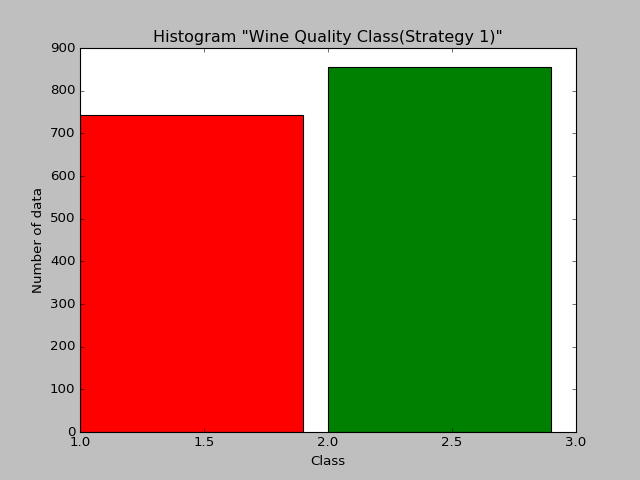
\includegraphics[width=0.6\linewidth,angle=0]{logo/label1.png}}\par}
\caption{ Labeling Strategy 1}
\end{figure}
{\centering{\bf{ Histogram of Quality}}}
\end{center}

\newpage

\subsection{Labelling Strategy 2}

According to James Halliday from James Halliday Annual Wine Companion, he separate wine quality into 5 class which are:Outstanding wines, Highly recommended, Recommended, Acceptable and Others. Thus I separate the data into 5 class as he did.
\begin{itemize}
\item{Class 1:  Quality in range [3, 4].}
\item{Class 2:  Quality equals 5}
\item{Class 3:  Quality equals 6}
\item{Class 4:  Quality equals 7}
\item{Class 5:  Quality equals 8}
\end{itemize}

The final labelling result is:

\begin{itemize}
\item{Class 1: 63 cases.}
\item{Class 2: 681 cases.}
\item{Class 3: 638 cases.}
\item{Class 4: 199 cases.}
\item{Class 5: 199 cases.}
\end{itemize}

\begin{center}
\begin{figure}[hbtp]
{\centering {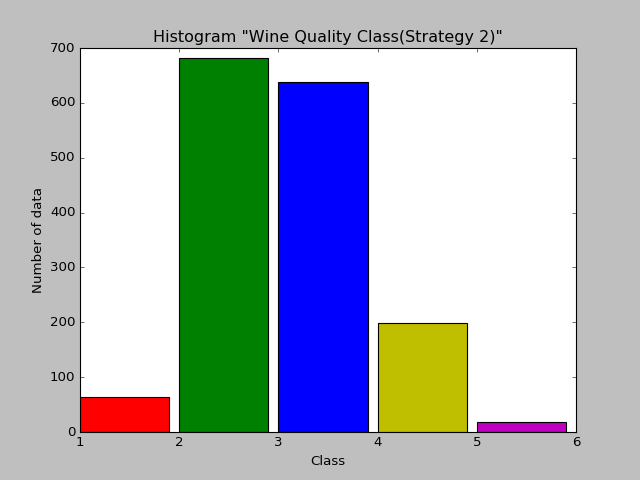
\includegraphics[width=0.6\linewidth,angle=0]{logo/label2.png}}\par}
\caption{ Labeling Strategy 2}
\end{figure}
{\centering{\bf{ Histogram of Alcohol}}}
\end{center}


\newpage

\section{Visualization}

\subsection{Principal Component Analysis}


After normalization, the co-variance of matrix $\mathcall{X}$ can be estimated as:
$$
\begin{align}
  \widehat{C_{j,k}} &= \frac{1}{N} \sum_{i=1}^{N} (x_j^i - \mu _j) \cdot (x_k^i - \mu_k) = \frac{1}{N} \sum_{i=1}^{N} x_j^i \cdot x_k^i \\
  \implies \widehat{C} &= \frac{1}{N}XX^T
\end{align}
$$

If the  ${\mathop{\mathbb{Cov}[X,Y]}}$ result is positive, that means that X,Y are positively correlated. The large the ${\mathop{\mathbb{Cov}[X,Y]}}$ result is, the dependency between X and Y will be.

After ${\mathop{\mathbb{Cov}[X]}}$ calculated, \code{linalg.eig()} function in \code{numpy} was called to generate the eigenvalues, eigenvectors of the co-variance matrix.

Once finish SVD decomposition, $\widetilde{\mathop{\mathbb{Cov}[X]}}$ can be calculated as a matrix whose diagonal elements are exactly the eigenvalues of ${\mathop{\mathbb{Cov}[X]}}$.

Many of the features here are related to class tags, but there is noise or redundancy. In this case, a feature dimensionality reduction method is needed to reduce the number of features, reduce noise and redundancy, and reduce the possibility of over-fitting.

The idea of PCA is to map n-dimensional features to the k dimension (k<n), which is a new orthogonal feature.This k-dimensional feature is called the pivot element, and it is a reconstructed k-dimensional feature, rather than simply removing the k dimension features from the n-dimensional feature

\newpage

\begin{center}
\begin{figure}[h]
{\centering {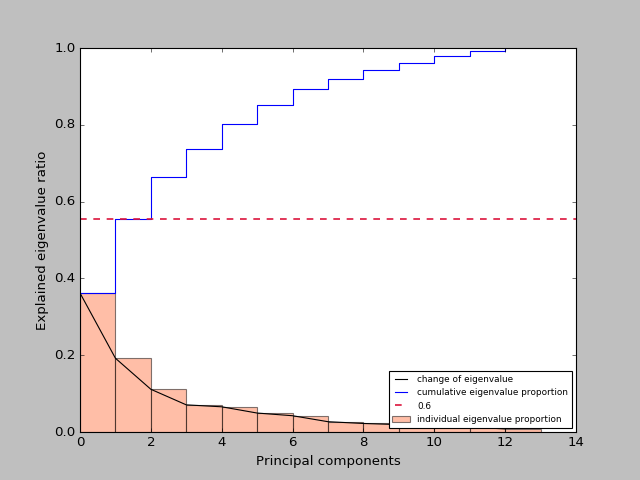
\includegraphics[width=0.7\linewidth,angle=0]{logo/2D_eigen_ratio.png}}\par}
\end{figure}
{\centering{\bf{Figure 1.3.1: Cumulative Eigenvalues of Co-variance Matrix}}}
\end{center}

\begin{center}
\begin{figure}[h]
{\centering {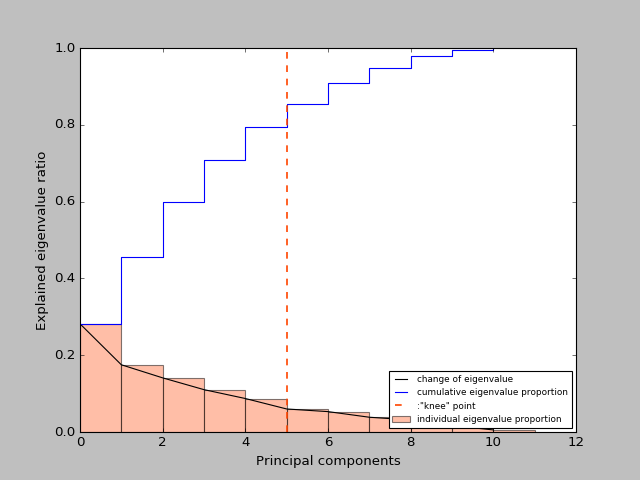
\includegraphics[width=0.7\linewidth,angle=0]{logo/knee_point.png}}\par}
\end{figure}
{\centering{\bf{Figure 1.3.2: Knee Points}}}
\end{center}

\newpage

The above  {\bf{Figure 1.3.1}} shows the cumulative eigenvalues of the co-variance matrix. It illustrates that if we just take two principal components base on this data set, it would not represent the original data set  roughly. Hence, in the {\bf{Figure 1.3.1}}, the knee point can be found according to the decrease ratio as the figure present.

The most important and useful information from PCA is the ranked imporance for the attributes.  It means how many separable or variance information is allocated in a certain attribute from the dataset.  In the following table, I list the value of the first 2 eigenvectors of the covariance matrix. The first column here shows coefficients of linear combination that defines principal component #1, and the second column shows coefficients for principal component #2. 

If the value is positive, there is a positive correlation between the value and the principal component it project to. While, if it is negative, things will opposite the positive one. However, whatever the sign of a value is, I just care about how large the absolute value it will be.  The large the absolute value is, the large effect it will do to principal component.


\begin{center}
{\centering{\begin{tabular}{ |l|l|l|l| }
  \hline
  \multicolumn{4}{|c|}{Top 2 Largest Eigenvalues and Eigenvectors} \\
  \hline
  \multicolumn{2}{|c|}{1st largest: 3.09913244} &
  \multicolumn{2}{|c|}{2nd largest: 1.92590969} \\
  \hline
  Dimensions & Values & Dimensions & Values\\
  \hline
  fixed acidity & 0.48931421519678553 & density & 0.5694869591070468\\
  citric acid & 0.4636316563339583 & total sulfur dioxide & -0.5236044991201001\\
  sulphates & -0.43851962406530764 & volatile acidity & 0.3986719794517932\\
  pH & 0.3953530087692868 & density & -0.37857017927744485\\
  alcohol & 0.242921330946993 & 'chlorides' & 0.20275695801841312\\
  volatile acidity & -0.23858436259606988 & citric acid & -0.1691026594058847\\
  chlorides & 0.21224658194729165 & sulphates & -0.1637023809766136\\
  residual sugar& 0.14610715358517834 & residual sugar & 0.10175002720609787\\
  total sulfur dioxide & -0.11323206500149913 & pH & -0.07645796788428783\\
  free sulfur dioxide & -0.036157524410518845 & free sulfur dioxide & 0.055788721251921254\\
  density & 0.023574853564211597 &  fixed acidity  & 0.04560728999309162\\
  \hline
\end{tabular}}}
{\centering{\bf{Table 1.3.1: Top two eigenvectors}}}
\end{center}

\newpage

Analysing the {\bf{Table 1.3.1: Top two eigenvectors}} In new axis 1,{\bf fixed acidity} index is the most important part because the coeffcient is {\bf 0.48931421519678553}which do largest contribution to the {\bf 1st principal component}. Similarly, {\bf density} is the most important part of {\bf 2 nd principal component} which is {\bf 0.5694869591070468}.
Combine with two column as the table display. We can only find that just {\bf residual sugar} appear in the {\bf last four value} both in 1st and 2 nd column. Thus, probably {\bf residual sugar} is the most useless feature in all data set.

\newpage

\begin{center}
\begin{figure}[h]
{\centering {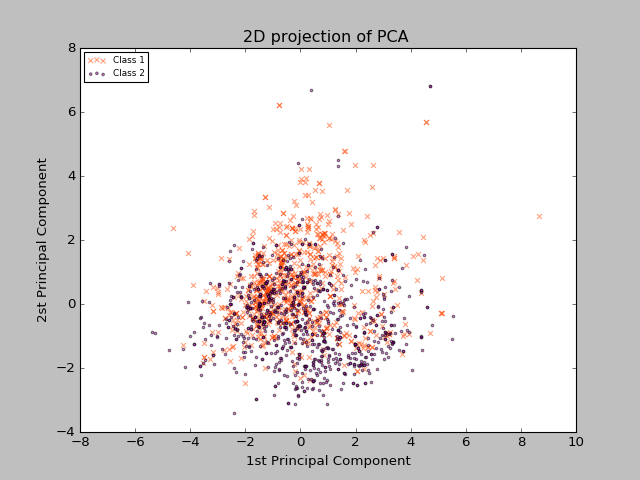
\includegraphics[width=0.7\linewidth,angle=0]{logo/2D_PCA.png}}\par}
\end{figure}
{\centering{\bf{Figure 1.3.3: 2D PCA projection }}}
\end{center}


\begin{center}
\begin{figure}[h]
{\centering {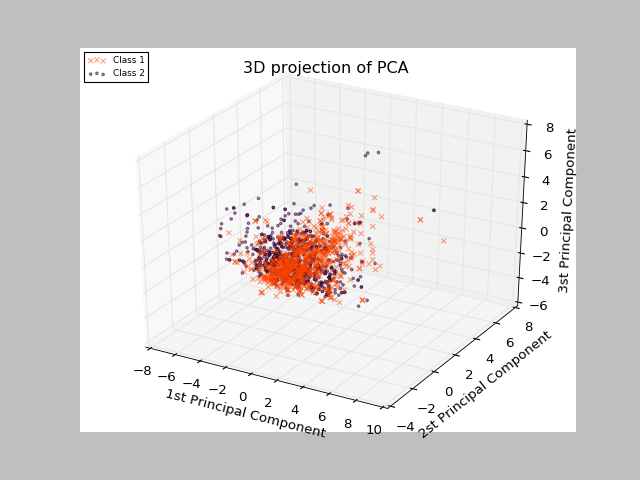
\includegraphics[width=0.7\linewidth,angle=0]{logo/3D_PCA_ex_quality.png}}\par}
\end{figure}
{\centering{\bf{Figure 1.3.4: 3D PCA projection of area }}}
\end{center}

\newpage

\begin{center}
\begin{figure}[h]
{\centering {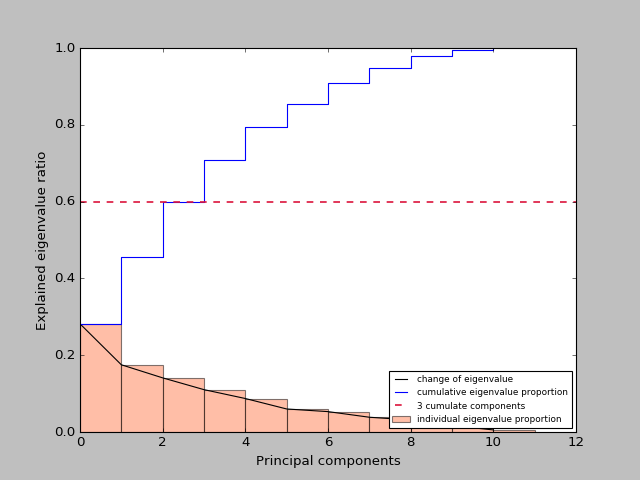
\includegraphics[width=0.7\linewidth,angle=0]{logo/3D_eigen_ratio.png}}\par}
\end{figure}
{\centering{\bf{Figure 1.3.5:  Ratio of 3 cumulative components}}}
\end{center}

\newpage


\subsection{Self-organizing Map}

To compare directly put original data set to som method and som after pca, I do the directly som firstly.

It is quite clear that the data be separated into two region, but actually we want to see the data can be analysis or observe in the lower dimension.  Directly som seems to reduce the dimension, however it is a {\bf fake}.  With the check of  normal vectors of the grids most of the cos value of the normal vectors are negative values or very small values, which means that the angle between each grid is pretty large, which confirm my judgement.


\begin{center}
\begin{figure}[h]
{\centering {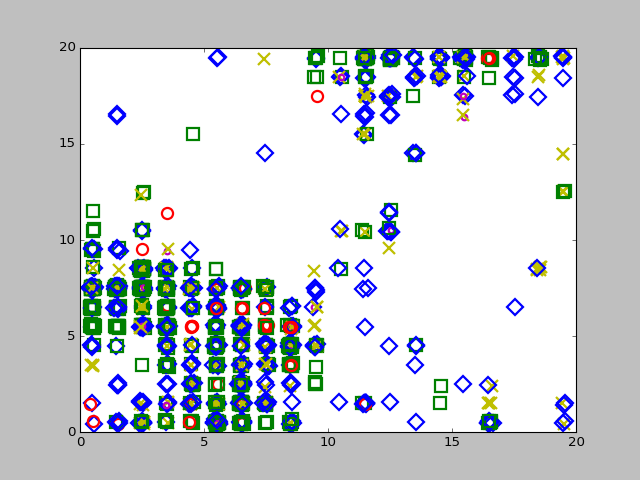
\includegraphics[width=0.7\linewidth,angle=0]{logo/direct_som.png}}\par}
\end{figure}
{\centering{\bf{Figure 1.3.5: Direct SOM of 11 Dimensional data }}}
\end{center}

\newpage

Next, I used PCA to make the data reduce to {\bf 5 dimensions} with the use of  label strategy 2. Here, the figure cover iteration 10times, 30 times, 50times.

\begin{center}
\begin{figure}[h]
{\centering {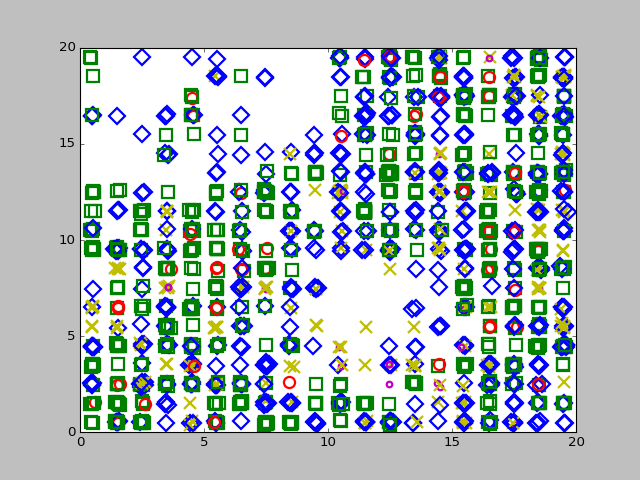
\includegraphics[width=0.7\linewidth,angle=0]{logo/2D_SOM_10.png}}\par}
\end{figure}
{\centering{\bf{Figure 1.3.6: SOM (Iteration: 10 times)}}}
\end{center}

\begin{center}
\begin{figure}[h]
{\centering {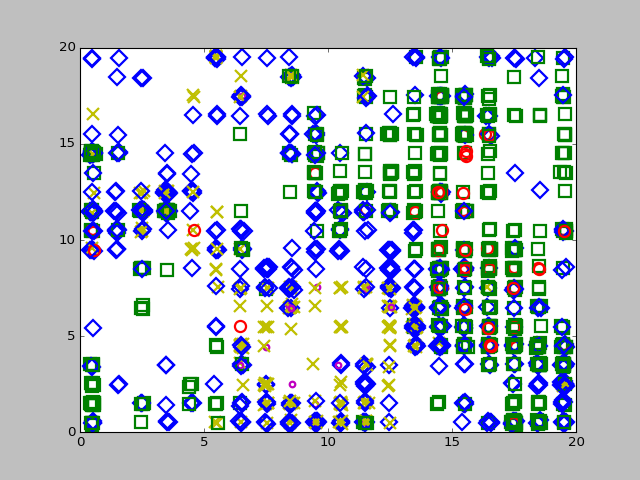
\includegraphics[width=0.7\linewidth,angle=0]{logo/2D_SOM_30.png}}\par}
\end{figure}
{\centering{\bf{Figure 1.3.7: SOM(Iteration: 30 times) }}}
\end{center}

\newpage

\begin{center}
\begin{figure}[h]
{\centering {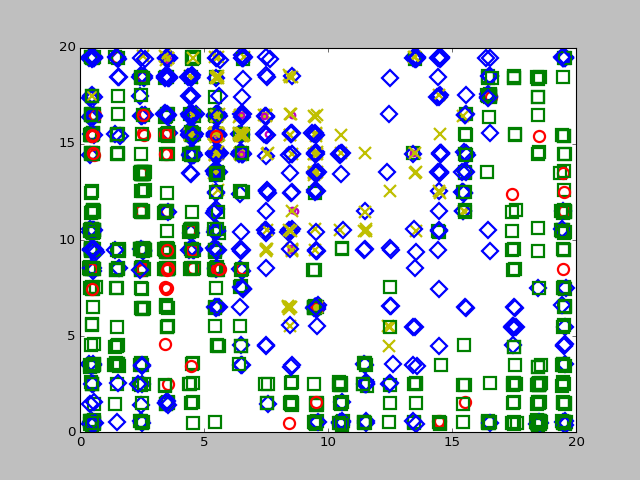
\includegraphics[width=0.7\linewidth,angle=0]{logo/2D_SOM_50.png}}\par}
\end{figure}
{\centering{\bf{Figure 1.3.7: SOM(Iteration: 50 times) }}}
\end{center}

\begin{center}
\begin{figure}[h]
{\centering {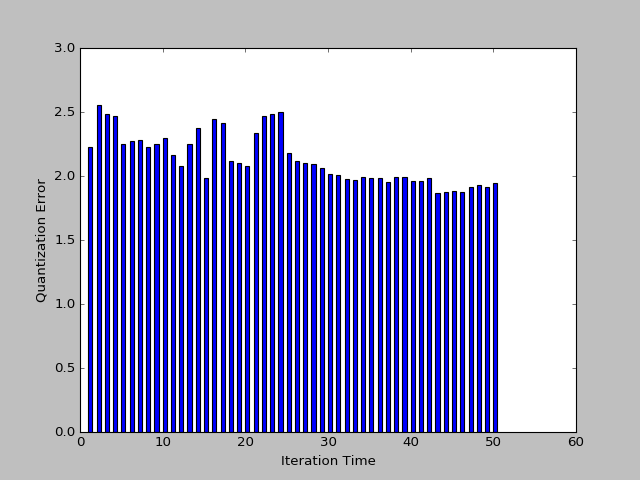
\includegraphics[width=0.7\linewidth,angle=0]{logo/SOM_quantization_error.png}}\par}
\end{figure}
{\centering{\bf{Figure 1.3.7: SOM Quantization Error) }}}
\end{center}

In conclusion, SOM can reduce the high level dimension data set to lower level dimension which will make us easier to see the data feature in the current lower coordinate. Although in some coordinate there exist some small cluster be separated,  we can find the link of nodes with same label dominate to whole graph.  And we can simply find the the data be separated into {\bf mainly 3 clusters: yellow, green, blue}.


\newpage

\subsection{The Comparision PCA and SOM}

PCA and SOM are different technique to reduce the dimension of data. There exist some common and difference between them. My conclusion is as follow.

\begin{itemize}
\item{When we focus a data set with {\bf high dimension}. If we want to reduce the dimension, we {\bf should not use SOM alone}. We should use PCA first to reduce the dimension as your wish, then do the SOM to make it easier to see the data feature in the current lower coordinate.}
\item{Both of them can reduce the dimension of data. However SOM is more likely to use for compressing and stretching the data to suit the new coordinate. PCA can just combine the current related dimension of  coordinate to form a new coordinate which is rather than a projection but a  combination. }
\end{itemize}

\newpage

\section{Clustering}
According to the conclusion of SOM after PCA, we simply find that there exist 3 clusters in the data set.

In order to find the difference of clustering with and without PCA, here I made a contrast group as follow.


\subsection{Clustering Without PCA}

\begin{center}
\begin{figure}[h]
{\centering {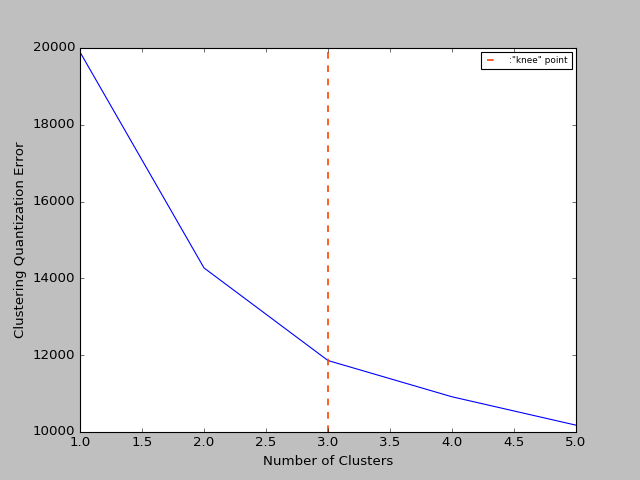
\includegraphics[width=0.7\linewidth,angle=0]{logo/knee_point_without_pca.png}}\par}
\end{figure}
{\centering{\bf{Figure 1.4.1:Clustering Quantization Error without PCA}}}
\end{center}

\newpage


\begin{center}
\begin{figure}[h]
{\centering {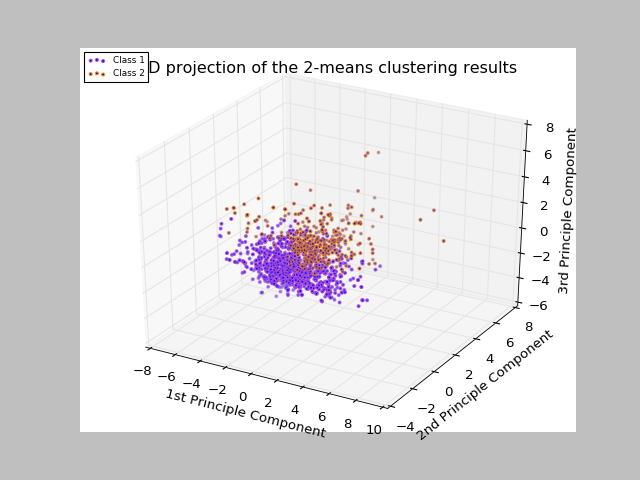
\includegraphics[width=0.7\linewidth,angle=0]{logo/3D_2-means_clustering.png}}\par}
\end{figure}
{\centering{\bf{Figure 1.4.2: 2-Means Clustering }}}
\end{center}

\begin{center}
\begin{figure}[h]
{\centering {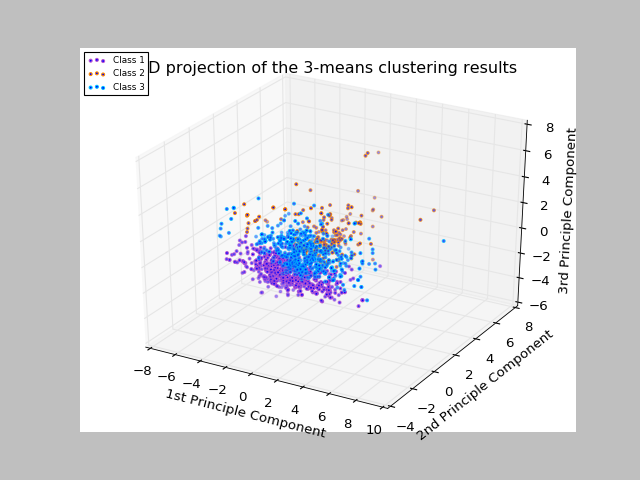
\includegraphics[width=0.7\linewidth,angle=0]{logo/3D_3-means_clustering.png}}\par}
\end{figure}
{\centering{\bf{Figure 1.4.3: 3-Means Clustering }}}
\end{center}

\newpage

\begin{center}
\begin{figure}[h]
{\centering {\includegraphics[width=0.7\linewidth,angle=0]{logo/3D_4-means_clustering.png}}\par}
\end{figure}
{\centering{\bf{Figure 1.4.4: 4-Means Clustering }}}
\end{center}

\begin{center}
\begin{figure}[h]
{\centering {\includegraphics[width=0.7\linewidth,angle=0]{logo//3D_4-means_clustering.png}}\par}
\end{figure}
{\centering{\bf{Figure 1.4.5: 5-Means Clustering }}}
\end{center}

{\bf Conclusion: Without doing the pca, the data we observe in the 3D level always aim to cover themselves. So that we can obsever the data straight forward which is not a good method.

\newpage


\subsection{Clustering with PCA}

We have see the result of clustering without pca. It seems not be a good method to obsever.  Hence, I try to do PCA first to reduce the dimension of data, to see if it can improve the observation.

\begin{center}
\begin{figure}[h]
{\centering {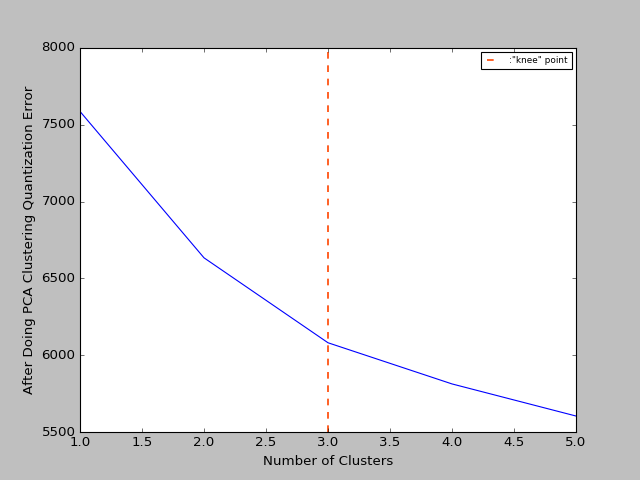
\includegraphics[width=0.7\linewidth,angle=0]{logo/knee_point_after_pca.png}}\par}
\end{figure}
{\centering{\bf{Figure 1.4.6: Clustering Quantization Error with PCA}}}
\end{center}

\newpage


\begin{center}
\begin{figure}[h]
{\centering {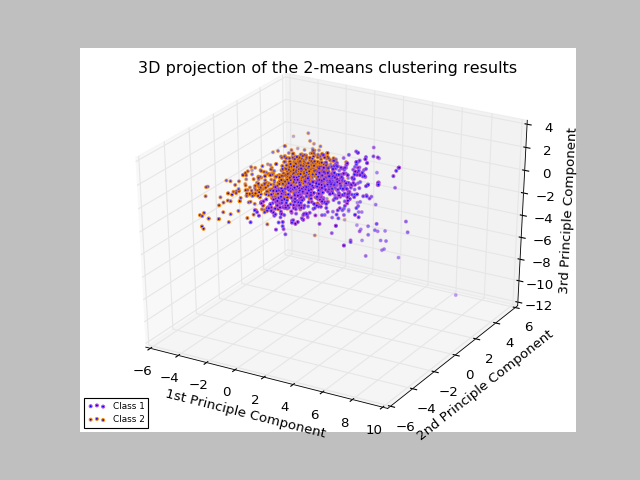
\includegraphics[width=0.7\linewidth,angle=0]{logo/3D_2-means_pca_clustering.png}}\par}
\end{figure}
{\centering{\bf{Figure 1.4.7: 2-Means Clustering }}}
\end{center}


\begin{center}
\begin{figure}[h]
{\centering {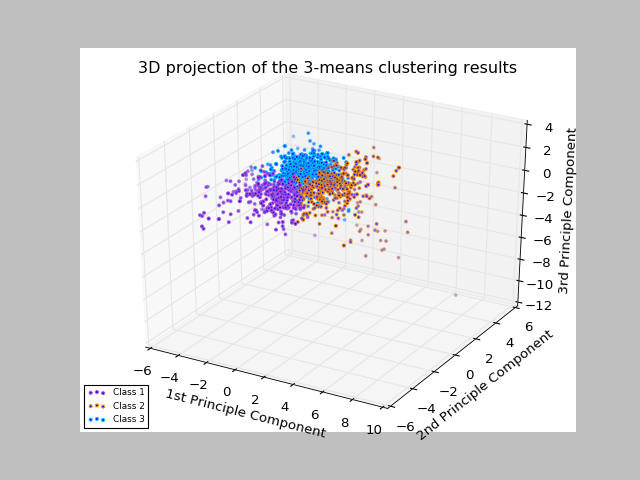
\includegraphics[width=0.7\linewidth,angle=0]{logo/3D_3-means_pca_clustering.png}}\par}
\end{figure}
{\centering{\bf{Figure 1.4.8: 3-Means Clustering }}}
\end{center}
\newpage


\begin{center}
\begin{figure}[h]
{\centering {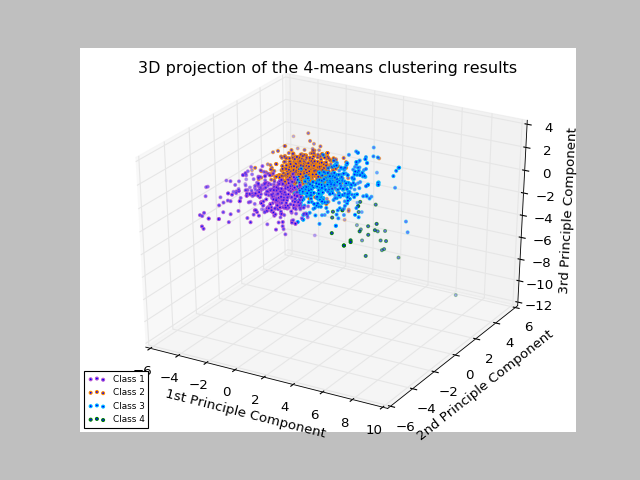
\includegraphics[width=0.7\linewidth,angle=0]{logo/3D_4-means_pca_clustering.png}}\par}
\end{figure}
{\centering{\bf{Figure 1.4.9: 4-Means Clustering }}}
\end{center}

\begin{center}
\begin{figure}[h]
{\centering {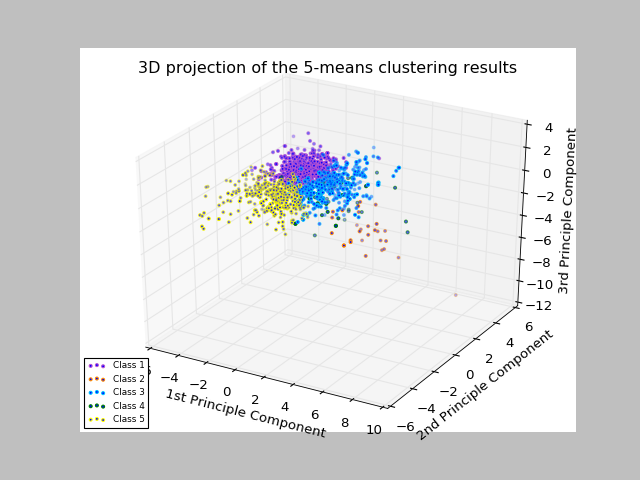
\includegraphics[width=0.7\linewidth,angle=0]{logo/3D_5-means_pca_clustering.png}}\par}
\end{figure}
{\centering{\bf{Figure 1.4.10: 5-Means Clustering }}}
\end{center}


\newpage

\subsection{Conclusion}

After  doing the clustering with or without PCA, my conclusion as follow.

Comparing the knee point in {\bf Figure 1.4.1} and {Figure 1.4.6}. It is obvious that {\bf clustering with PCA reduce the quantization error}. It might because of the reduction of dimension the PCA have done simultaneously reduce the noise.
The knee point in graph of quantization error can not be a judgement of result of clustering. So we see the {\bf Figure 1.4.8} to estimate if this clustering method is suitable to this data set. We can find that the data set be separated unambiguous. Thus, k-means clustering is suitable for this data set.


\newpage




\chapter{If there are any attribute that influence total sulfur dioxide?}

\section{Labelling}

Strategy of labelling the total sulfur dioxide (0,160], (160 440]

\section{Visualization}

\subsection{Principal Component Analysis}

Just like what I did in {\bf{Section 1.3}}, I used the same technique to complete this part. 
The result as follow. The first two feature affect to the data are fixed acidity and alcohol, which are {\bf 0.48809550387543194} and {\bf  -0.5528903530300658}


\begin{center}
{\centering{\begin{tabular}{ |l|l|l|l| }
  \hline
  \multicolumn{4}{|c|}{Top 2 Largest Eigenvalues and Eigenvectors} \\
  \hline
  \multicolumn{2}{|c|}{1st largest: 3.12113839} &
  \multicolumn{2}{|c|}{2nd largest: 2.11175471} \\
  \hline
  Dimensions & Values & Dimensions & Values\\
  \hline
  fixed acidity & 0.48809550387543194 & alcohol & -0.5528903530300658\\
  citric acid & 0.4734325262220812 & quality & -0.5236044991201001\\
  pH & -0.4326046485510123 & volatile acidity & 0.3986719794517932\\
  density & 0.3698915265676169 & density & -0.37857017927744485\\
  volatile acidity & -0.2655231833551456 & 'chlorides' & 0.20275695801841312\\
  sulphates & -0.2545312162478427 & citric acid & -0.1691026594058847\\
  chlorides & 0.19715263821767132 & sulphates & -0.1637023809766136\\
  residual sugar & 0.13860211721461613 & residual sugar & 0.10175002720609787\\
  quality & 0.11318644768411748 & pH & -0.07645796788428783\\
  alcohol & -0.07242073902021279 & free sulfur dioxide & 0.055788721251921254\\
  free sulfur dioxide & -0.047260478851762794 &  fixed acidity  & 0.04560728999309162\\
  \hline
\end{tabular}}}
{\centering{\bf{Table 2.3.1: Top two eigenvectors}}}
\end{center}

\newpage

\begin{center}
\begin{figure}[h]
{\centering {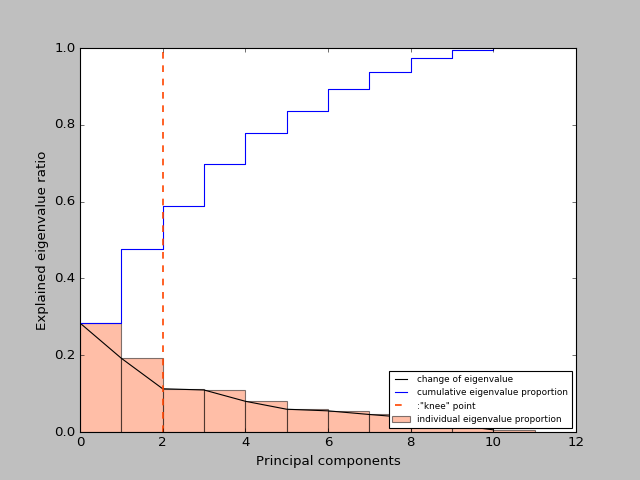
\includegraphics[width=0.7\linewidth,angle=0]{logo/knee_point_2.png}}\par}
\end{figure}
{\centering{\bf{Figure 2.3.1: Cumulative eigenvalues of co-variance matrix}}}
\end{center}


\newpage

\begin{center}
\begin{figure}[h]
{\centering {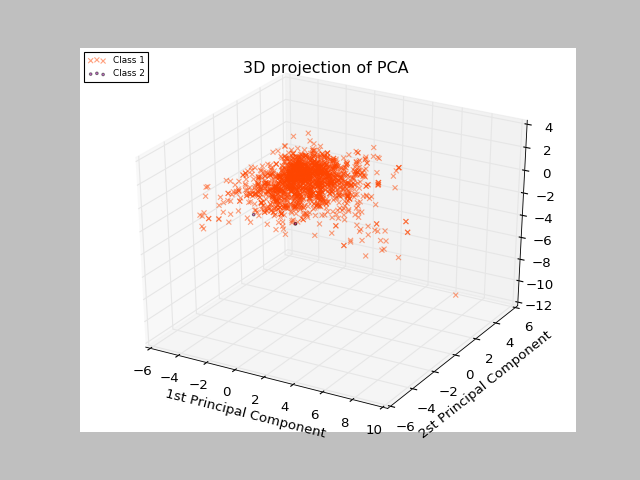
\includegraphics[width=0.7\linewidth,angle=0]{logo/3D_PCA_ex_sulfur.png}}\par}
\end{figure}
{\centering{\bf{Figure 2.3.4: 3D PCA projection of total sulfur dioxide }}}
\end{center}


\begin{center}
\begin{figure}[h]
{\centering {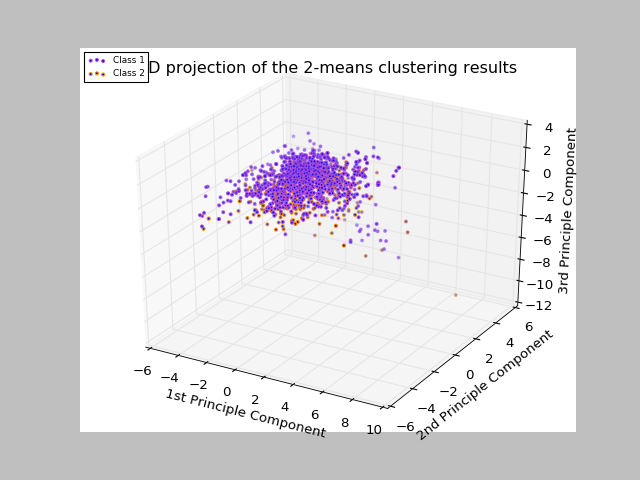
\includegraphics[width=0.7\linewidth,angle=0]{logo/3D_2-means_clustering_2.png}}\par}
\end{figure}
{\centering{\bf{Figure 2.3.4: Clustering of total sulfur dioxide }}}
\end{center}
\newpage

\section{Conclusion}

As what I  mention, The first two feature affect to the total sulfur dioxide are fixed acidity and alcohol, which are {\bf 0.48809550387543194} and {\bf  -0.5528903530300658}

Because of the limitation of working time and similarity of works, SOM and clustering were only present one figure.

However, I cover all the requirements.

If it is possible, I am looking forward to be your students in the future. 

Finally, I sincerely express my thanks here to GuoJi and Peter.
\vspace*{0.5cm}\\
{\large \bf {Code \& Related Files:}}
\newline{}
{\hspace*{0.7cm}{\url{https://github.com/Voldet/data_analysis}} }

\bibliographystyle{plain}
\bibliography{cimne}
\end{document}
